\documentclass{article}
\usepackage[a4paper, left=2cm,right=2cm,top=2.5cm,bottom=2cm]{geometry}
\usepackage[utf8]{inputenc}
\usepackage[english]{babel}
\usepackage{natbib}
\usepackage{graphicx} % Required for inserting images
\usepackage{amsmath,amsthm,amssymb}
\usepackage{braket}
\usepackage{tikz}
\usepackage{qcircuit}
\newtheorem{theorem}{Theorem}
\usepackage{subcaption}



\usepackage{bm}        
\usepackage{booktabs}

\usepackage{mathtools}
\DeclarePairedDelimiterX\ketbra[2]{\delimsize\vert}{\delimsize\vert}{#1\rangle\langle#2}


\usepackage{xcolor}
\usepackage[colorlinks = true,
            linkcolor = blue,
            urlcolor  = blue,
            citecolor = blue,
            anchorcolor = blue]{hyperref}


%%% New Commands
\newcommand{\dd}{\mathrm{d}}
\newcommand{\Cbb}{\mathbb{C}}
\newcommand{\Rbb}{\mathbb{R}}
\newcommand{\Tcal}{\mathcal{T}}
\newcommand{\Ocal}{\mathcal{O}}
\newcommand{\N}{\mathbb{N}}
\newcommand{\Z}{\mathbb{Z}}
\newcommand{\R}{\mathbb{R}}
\newtheorem{remark}{Remark}
\newtheorem{assumption}{Assumption}

\newcommand{\cb}[1]{{\color{blue}#1}}
\newcommand{\cr}[1]{{\color{red}#1}}

%%%%%%%%%%%%%%%%%%%%%%%%%%%%%%%%%%%%%%%%%%%%%%%%%%%%%%%%%%%%%%%%%%%%%%%%%%%%%%%%%%%%%%%%%%%%%%%%%%%%%%%%%%%%%%%%%%%%%%%



\title{Quantum Differential Equation Solver via Hybrid Oscillator-Qubit Linear Combination of Hamiltonian Simulations}
\author{Elin Ranjan Das, Muqing Zheng, Rishab Dutta, Ang Li, Yuan Liu}
\date{August 2025}


\begin{document}

\maketitle

\begin{abstract}
    We propose an advanced method for quantum simulation based on the linear combination of Hamiltonian simulation (LCHS) within a hybrid oscillator-qubit architecture. This approach capitalizes on the inherent advantages of continuous (oscillator) and discrete (qubit) variables, eliminating the need for discretization and the associated truncation errors commonly found in discrete variable LCHS. This work marks an important step forward in overcoming the limitations of traditional simulation methods and advancing the capabilities of quantum computing.
\end{abstract}

%%%%%%%%%%%%%%%%%%%%%%%%%%%%%%%%%%%%%%%%%%%%%%%%%%%%%%%%%%%%%%%%%%%%%%%%%%%%%%%%%%%%%%%%%%%%%%%%%%%%%%%%%%%%%%%%%%%%%%%









%%%%%%%%%%%%%%%%% Introduction Starts %%%%%%%%%%%%%%%%%%%%%
\section{Introduction}

The ability of controllable quantum systems to efficiently emulate complex quantum dynamics has motivated substantial theoretical and experimental efforts. Accurate simulation of quantum many-body systems underpins advances in condensed matter physics, quantum chemistry, high-energy physics, and materials science~\cite{Clinton_2024}. However, realizing scalable and precise quantum simulation remains a central challenge due to hardware limitations and algorithmic constraints.

One of the most powerful algorithmic paradigms for digital quantum simulation is Hamiltonian simulation via linear combinations of unitaries (LCU)~\cite{2012}. In this framework, the target Hamiltonian is decomposed into a weighted sum of efficiently implementable unitary operators, enabling high-precision time evolution with provable complexity bounds. Building on this idea, linear combination of Hamiltonian simulation (LCHS)~\cite{LCHS1,LCHS2} methods provide a systematic way to construct evolution operators while maintaining controllable error scaling. However, existing implementations of LCHS rely exclusively on discrete-variable (qubit-based) architectures, where continuous degrees of freedom must first be discretized. This discretization introduces truncation errors and often requires large qubit overhead to achieve high fidelity, particularly when simulating systems with inherently continuous variables.

Continuous-variable (CV) quantum systems such as harmonic oscillators realized in photonic modes or superconducting cavities naturally encode infinite-dimensional Hilbert spaces. These systems are well suited for representing bosonic modes and field-theoretic models without the need for coarse discretization. Meanwhile, qubit-based platforms provide strong nonlinearity, robust control, and efficient implementation of conditional operations. Hybrid oscillator-qubit architectures combine the advantages of both paradigms, offering expanded computational expressiveness and improved resource efficiency.

In this work, we propose an advanced method for quantum simulation based on linear combination of Hamiltonian simulation within a hybrid oscillator-qubit architecture. By leveraging continuous-variable encodings for naturally bosonic degrees of freedom and discrete-variable control for selective unitary operations, our approach eliminates the discretization step that typically introduces truncation errors in purely qubit-based LCHS implementations. The resulting framework enables more faithful representation of continuous dynamics while preserving the algorithmic strengths of linear-combination-based simulation techniques.






%%%%%%%%%%%%%%%%% Motivation Starts %%%%%%%%%%%%%%%%%%%%%






\section{Motivation}







LCHS provides an optimal state preparation cost and a near-optimal scaling in matrix queries on all parameters for solving linear ordinary differential equations (ODEs) in the form of
\begin{align}
    \frac{\dd u(t)}{\dd t} = -A(t)u(t) + b(t), \quad u(0) = u_0  \label{eq:lchs-ODE}
\end{align}
where $t \in [0, T]$, $A(t) \in \Cbb^{N \times N}$ and $u(t), b(t) \in \Cbb^{N}$. The solution of the ODE~\eqref{eq:lchs-ODE} has the explicit form
\begin{align}
    u(T) &= \Tcal e^{- \int^T_0 A(s) \dd s}u_0 + \int^T_0 \Tcal e^{-\int^T_s A(s')\dd s'}b(s) \dd s \label{eq:exp-sol}
\end{align}
where $\Tcal$ is the time-ordering operator. To start with, the coefficient matrix $A(t)$ is first decomposed into \[A(t) = L(t) + iH(t)\] via Cartesian decomposition \[L(t) = \frac{A(t) + A^\dagger(t)}{2}, H(t) = \frac{A(t) - A^\dagger(t)}{2i}.\] It is assumed that $L(t) \succeq 0$. Otherwise, we can shift the eigen spectrum of $u(t)$ by substituting $u(t) = e^{ct}v(t)$ and use $v(t)$ for the ODE system so that $L(t) + cI \succeq 0$, where $-c$ is the minimum of the smallest eigenvalues of $L(t)$. LCHS provides that 
\begin{align}
    \Tcal e^{- \int^t_0 A(s) \dd s} &= \int_{\Rbb}  g(k) \left[\Tcal e^{-i \int^t_0 (kL(s)+H(s))\dd s} \right] \dd k \label{eq:LCHS-sol-homo} \\
    \int^t_0 \Tcal e^{-\int^t_s A(s')\dd s'}b(s) \dd s &= \int^t_0 \int_\Rbb g(k) \left[ \Tcal e^{-i \int^t_s (kL(s')+H(s'))\dd s'} \right]  b(s) \dd k \dd s   \label{eq:LCHS-sol-inhomo}
\end{align}
where $g(k):=\frac{f(k)}{1-ik}$ for some kernel function $f(k)$ and $t \in [0,T]$. The choice of $f(k)$ that leads to near-optimal complexity dependency on all parameters is $f(k) = \frac{e^{2^{\beta}}}{2\pi e^{(1+ik)^\beta}}$, where $\beta \in (0,1)$ is a user-defined constant~\cite{LCHS2}.
Note that the terms in brackets in Eq.~\eqref{eq:LCHS-sol-homo} and~\eqref{eq:LCHS-sol-inhomo} are unitary. Thus, LCHS further truncates and discretizes the integrals in Eq.~\eqref{eq:LCHS-sol-homo} and~\eqref{eq:LCHS-sol-inhomo} into a sum of unitaries, employing state preparation circuits for $\ket{u_0}:=\frac{u_0}{\|u_0\|}$ and $\ket{b(s)}:=\frac{b(s)}{\|b(s)\|}$ and the linear combination of unitaries (LCU) circuits to prepare the solution state $\ket{u(T)}:=\frac{u(T)}{\|u(T)\|}$~\cite{LCHS1,LCHS2}.




Combining with the finite difference method and linearization methods, for example, Carleman linearization~\cite{liu2021carleman}, various non-linear partial differential equations can also be converted into a linear ODE system that is solvable by LCHS. However, the number of terms in the discretized LCHS integral, denoted by $M$, brings a huge cost on quantum resources in the circuit implementation level for either near-term or early fault-tolerant quantum machines. For the complementary solution, $M$ has complexity
\begin{align*}
        M \in \Ocal\left( T \max_t \|L(t)\|\left(\log \frac{1}{\epsilon}\right)^{1+1/\beta} \right)
\end{align*}
where $\epsilon$ is the total error incurred by LCHS~\cite{LCHS2}. The corresponding LCU circuit requires $\lceil\log_2(M)\rceil$ ancillary qubits, and more problematically, $\lceil\log_2(M)\rceil$-controlled multiple-qubit unitary operators for Hamiltonian simulations. In this case, for a time-independent ODE, the value of $M$ can be in the $10^6$ magnitude when $\epsilon$ is around $10^{-5}$, $\beta=0.8$, $T=1000$, and $\|L\|=1$. More exact scalings of LCHS are provided in~\cite{pocrnic2025constant}. 




Inspired by the continuous LCU in~\cite{bell2025co}, a hybrid CV-DV LCHS is a promising direction to bring down the resource cost and, ideally, remove truncation and discretization errors in the integrals calculation. Specifically, continuous LCU can use $\Ocal(1)$ number of ancillary oscillators, along with CV state preparation and CV measurements, replace $\lceil\log_2(M)\rceil$ ancillary qubits in the DV LCU circuit, while the unitaries for Hamiltonian evolution remain in qubit space. Continuous LCU circuit can compute the integrals in Eq.~\eqref{eq:LCHS-sol-homo} and~\eqref{eq:LCHS-sol-inhomo} without truncation and discretization on integrals, whereas truncations errors may still persist in CV state preparation and hybrid Hamiltonian simulation.


% \textbf{Potential hardware.} Trapped-ion devices  (Duke Quantum Center?, Pagano Research Group in Rice) and cavity QED devices (Schuster lab in Standford), supporting Gaussian gates (displacement, phase rotation, squeezing) and non-Gaussian (SNAP)

% \textbf{Potential software.} Construct a customized backend package for LCHS on HybridLane











%%%%%%%%%%%%%%%%% Methdology Starts %%%%%%%%%%%%%%%%%%%%%





\section{Methodology}





Let us consider a time-independent homogeneous ODE system, where $A(t):=A$ and $b(t) := 0$ for all $t$. From Eq.~\eqref{eq:exp-sol} and~\eqref{eq:LCHS-sol-homo}, the complementary solution becomes
\begin{align}
    u(t) &= \left[\int_{\Rbb}  g(k)  e^{-i t (kL+H)}  \dd k \right] u_0 \label{eq:sol-homo-lchs}
\end{align}
for $t \in [0,T]$. Using a single oscillator for the ancillary in continuous LCU, the qubits that synthesize unitary $e^{-i t (kL+H)}$ need to couple with this ancillary oscillator, leading to the joint evolution
\(
    e^{-it ( L \otimes \hat{k} + H \otimes I)},
\)
where $\hat{k}$ is one of the canonical conjugation operators ($\hat x$ and $\hat p$) and $I$ is the identity operator. That is to say, the qumode remains untouched when $H$ acts on the qubit system. 

Before forming the circuit for the joint evolution, an appropriate function $g(k)$ has to be obtained. To do this, we need to prepare and post-select two appropriate CV states. 

Let \(\ket{\Psi}=\ket{\psi}_{\rm osc}\ket{u_0}_q\) be the preparation state, where $\ket{\psi}_{\rm osc}$ is the initial oscillator state and $\ket{u_0}$ is the initial qubit state. 
Let \(\bra{\Phi}=\bra{\phi}_{\rm osc}\otimes \mathbf{I}_q\) be the post-selection projector, where $\bra{\phi}_{\rm osc}$ acts only on the oscillator and the qubit remains untouched. 

If we choose the position operator $\hat x$ for $k$, then according to ref.~\cite{bell2025co}, the qumode sandwich gives
\begin{align}
     \bra{\Phi}  e^{-it ( \hat{x} \otimes L + \mathbf{I}_{\rm osc} \otimes H)} \ket{\Psi} = \bigg[\int_{\mathbb{R}} \dd x \, \phi^*(x) \psi(x)    e^{-it ( xL + H)}\bigg]\ket{u_0}_q.
\end{align}
Comparing to the Eq.~\eqref{eq:sol-homo-lchs}, this gives \(g(x)= \phi^*(x) \psi(x)\). Namely, we need to engineer the preparation and post-selection states to obtain an appropriate $g(x)$ that satisfies LCHS's requirements. 

We choose the post-selection state $\ket{\phi}$ to be a squeezed vacuum, whose position-space wavefunction is 
\begin{align}
    \phi_r(x):=S(r,0)\phi_0(x)=\bigg(\frac{2}{e^{2r}\pi}\bigg)^{1/4} e^{-x^2/e^{2r}}=\bigg(\frac{2}{\sigma^2\pi}\bigg)^{1/4} e^{-x^2/\sigma^2}
\end{align} 
with squeezing parameter $r$ and wavefunction standard deviation $\sigma=e^r$, and this gives the corresponding initial state to be prepared 
\begin{align}
    \psi_r(x):=\bigg(\frac{\sigma^2\pi}{2}\bigg)^{1/4}g(x)e^{x^2/\sigma^2}= \mathcal{N}g(x)e^{x^2/\sigma^2}.
\end{align}

This leads to our formulation of a CV/DV LCHS theorem:
\begin{theorem}[Continuous-discrete variable LCHS]
%     Suppose \(A(t) = L(t) + i H(t)\) and \(L(t) \succeq 0\), then
% \[
% \mathcal{T} e^{-\int_0^t A(s) \, ds} = \int_{\mathbb{R}} g(k) U_k(t) \, dk.
% \]
% Here $U_k(t)$ are unitaries that solve the Schr{\"o}dinger equation
% \[\frac{dU_k(t)}{dt}=-i(kL(t) + H(t))U_k(t);\qquad U(0) = I\]
% and \(g(z)=\frac{f(z)}{1-iz}\) is a function of \(z \in \mathbb{C}\), such that:
% \begin{enumerate}
%     \item \textbf{(Analyticity)} \(f(z)\) is analytic on the lower half plane \(\{z: \mathrm{Im}(z) < 0\}\) and continuous on \(\{z:\mathrm{Im}(z) \leq 0\}\),
%     \item \textbf{(Decay)} there exist \(\alpha > 0,~C > 0\) such that \(|z|^{\alpha} |f(z)| \leq C\) when \(\mathrm{Im}(z) \leq 0\),
%     \item \textbf{(Normalization)} \(\int_{\mathbb{R}} g(k)\dd k = 1\).
%     \item \textbf{(Square-integrability)} there exist $r\in \mathbb{R}_+$ such that \(\int_\mathbb{R}\dd k|f(k)|^2\frac{e^{2k^2/e^{2r}}}{1+k^2} <\infty\)
% \end{enumerate}
Suppose \(A = L + i H\) and \(L \succeq 0\), then $u(t)$ can be expressed as the following:
\begin{align}
    \ket{u(t)} = e^{-At} \ket{u(0)} &= \braket{\Phi| e^{-it ( \hat{x} \otimes L+ \mathbf{I}_{\rm osc} \otimes H )} |\Psi}\\ 
    &= (\bra{\phi}_{\rm osc}\otimes\mathbf{I}_q)  e^{-it ( \hat{x} \otimes L+ \mathbf{I}_{\rm osc} \otimes H )} (\ket{\psi}_{\rm osc}\otimes\ket{u_0}_q)\\
    &= \bigg[\int_{\mathbb{R}} \dd x \, \phi^*(x) \psi(x)    e^{-it ( xL + H)}\bigg]\ket{u_0}_q.
\end{align}


\textit{where $\ket{\psi}_{\rm osc}$ and $\ket{\phi}_{\rm osc}$ are squeezed Fock states.}
\end{theorem}

% In the coherent basis expansion,
% \begin{align*}
%     \ket{\psi}=\frac{1}{\pi}\int\dd^2\alpha\ket{\alpha}\braket{\alpha|\psi}\approx\frac{1}{\pi}\int\dd^2\alpha\braket{\alpha|\psi}\sum_{n=0}^{N_{\mathrm{max}}}\frac{\alpha^n}{\sqrt{n!}}\ket{n}
% \end{align*}
At this point, the missing piece for the whole hybrid CV-DV LCHS circuit is the oracle syntheses for matrices $L$ and $H$, whose basis-gate implementations are highly dependent on the structures of both matrices and are very problem-specific. Many previous works in the DV regime tackle this problem by decomposing coefficient matrices into linear combinations of Pauli matrices, for example, hyperbolic partial differential equations~\cite{PhysRevResearch.6.033246} and advection-diffusion equation~\cite{alipanah2025quantum}. Borrowing their designs and following the circuit synthesis in~\cite{bell2025co}, the evolution of decomposed Hamiltonians coupled with oscillators can be constructed in CV-DV circuits.








%%%%%%%%%%%%%%%%% Methodology-Statepreparation Starts %%%%%%%%%%%%%%%%%%%%%







\subsection{State Preparation}


\label{ss:state-prep}




We now consider two special cases of $\psi_r(x)$ preparation and their implications.
\begin{itemize}
    \item $\mathbf{r=0~(\sigma=1):}$ This leads to the post-selection state being the vacuum state $\phi_0(x)$. However, our preparation state becomes
    \begin{align}
        \psi_0(x) := \mathcal{N}g(x)e^{x^2}
    \end{align}
    which is not a physically realizable state, as $\psi_0(x)\notin L^2(\mathbb{R}).$ 
    
    This gives us an additional condition imposed on the $g(x)$ for CV-DV LCHS: 
    \begin{align}
        \exists\ r>0\ \text{s.t}\ \int_\mathbb{R} \dd x |g(x)|^2 e^{\frac{2x^2}{\sigma^2}} <\infty
    \end{align}

    \item $\mathbf{r\to\infty~ (\sigma\to\infty):}$ This leads to $\phi_r(x)$ being the infinitely squeezed vacuum state. Then our preparation state is simply the kernel itself:
    \begin{align}
        \psi_\infty(x) := \lim_{r\to\infty} \psi_r(x)= \mathcal{N}g(x)
    \end{align}
\end{itemize}
The initial state $\ket{\psi_r}$ can be approximated via a finite squeezed Fock expansion
\begin{align}
    \psi_r(x)&=\mathcal{N}g(x)e^{x^2/\sigma^2} \approx \sum_{{\mathfrak n} = 0}^{N} C_{\mathfrak n} \braket{x|S(r,0)|{\mathfrak n}}=\psi'(x)
\end{align}
where coefficients $\{C_{\mathfrak n}\}$ are overlaps
\begin{align}
    C_{\mathfrak n} &= \braket{{\mathfrak n}|S^\dagger(r',0)|\psi_r} = \int_{\mathbb{R}} \dd x \, \phi^*_{\mathfrak n}(x/\sigma')\,e^{-x^2/\sigma^2} \psi_r(x)
\end{align}
This expression simplifies to
\begin{align}
    C_{\mathfrak n}= \sqrt{\frac{\sigma}{\sigma'}}\frac{1}{\sqrt{2^{\mathfrak n}{\mathfrak n}!}}\int_{\mathbb{R}}\dd x\,  H_{\mathfrak n}(x/\sigma')g(x)e^{-\gamma x^2}
    &= \int_{\mathbb{R}}\frac{\dd x\, e^{2^\beta}H_{\mathfrak n}(x/\sigma')e^{-\gamma x^2}}{2\pi e^{{(1+ix)}^\beta}(1-ix)}
    \label{eq:coefficients}
\end{align}
where \(\gamma=\frac{1}{\sigma'^2}-\frac{1}{\sigma^2}=\frac{1}{e^{2r'}}-\frac{1}{e^{2r}},\quad r'<r\). While eq.~\eqref{eq:coefficients} can have analytical forms depending on specific values of $\beta,$ it is not possible to derive a generalized expression. Two examples of closed analytic form for the limit values of $\beta=\{0,1\}$ are given in~\ref{ss:analytic}.
\cr{The draft should not mix $\hbar=2$ and $\hbar=1$ conventions across sections.}
\cb{In this paper we take $\hbar=2$ as the standard convention, so the coefficient formula above is the paper-facing expression. The corresponding $\hbar=1$ translation used by the numerical backends is collected in the appendix for implementation convenience.}
















%%%%%%%%%%%%%%%% Methodology-Errorbound starts %%%%%%%%%%%%%%%%%%%%% Elin




\subsection{Error bound estimation for state preparation}

Ideally we want to realize $\psi_r(x)=g(x)e^{x^2/{e^{2r}}}$ as close as possible using Gaussian (Fock) states. Previously, authors from \cite{Jin_2024} showed that sub-optimal kernel function $f(k)=\frac{1}{\pi(1+ik)}$ could be realized with a squeezed vacuum state with maximum fidelity of 98.6\% with a squeezing parameter of 0.925. However, we show that the near-optimal kernel function can be realized instead with a superposition of squeezed Fock states for arbitrary closeness, where the approximation error is bounded by the Fock cutoff level (or the oscillator energy) and the squeezing parameter:

\begin{theorem}
\label{thm: state-prep}
Let $\psi_r(k)$ denote the ideal prepared state, and let $\psi'(k)$ be an
$\epsilon_s$-approximation to $\psi_r(k)$. Then for any $\epsilon_s>0$,
there exist a Fock cutoff $N\in\mathbb{N}$ and a squeezing parameter $r>0$
such that
\[
\|\psi'-\psi_r\| < \epsilon_s .
\]
Moreover, the required resources scale asymptotically as
{\color{red}
\[
N = \mathcal O\!\left(\log^2 \frac{1}{\epsilon_s}\right),
\qquad
r = \Omega\!\left(\log \frac{1}{\epsilon_s}\right).
\]
}
\cb{For this proof strategy these are sufficient choices, so the theorem statement should instead read}
{\color{blue}
\[
N = \mathcal O\!\left(\log^2 \frac{1}{\epsilon_s}\right),
\qquad
r = \mathcal O\!\left(\log \frac{1}{\epsilon_s}\right).
\]
}
\end{theorem}


\begin{proof}
    Let \(\mathbb{H}_N = \text{span}\{\psi_{\mathfrak n}\}_{{\mathfrak n}=0}^N\) denote the truncated bosonic Hilbert space spanned by the squeezed Fock basis $\psi_{\mathfrak n}$, and let \(\Pi^F_N : L^2(\mathbb{R}) \to \mathbb{H}_N\) be the orthogonal projection. Define the truncated approximation as the projection of \(g\), 
    \[
    \Pi^F_Ng = \sum_{{\mathfrak n}=0}^N C_{\mathfrak n} \psi_{\mathfrak n} = \psi'.
    \]  
    The ideal prepared state is $\psi_r(k) = g(k) e^{k^2 e^{-2r}}$.
    
    Using the triangle inequality,
    $$\lVert \psi' -\psi_r\rVert\leq \lVert g - \Pi_N^F g\rVert + \lVert g - g e^{k^2 e^{-2r}}\rVert =: \tau(N) + \delta(r).$$
    We estimate the two contributions separately.
    
    $g$ is analytic in the strip  
        \(\mathcal{S}_{\rho} := \{ z \in \mathbb{C} : \Im(z) \in [-\rho, \rho] \}\) for some \(\rho=1-\epsilon\) with \(\epsilon\to0\).
    Then the convergence analysis of Hermite approximations~\cite[Thm.~3.8]{wang2025convergenceanalysishermiteapproximations}\footnote{The strict version of the theorem states that $g$ must satisfy some growth conditions as well. However, the authors imply in the same work that the growth conditions can be relaxed \cite[pp.~15]{wang2025convergenceanalysishermiteapproximations}. Here we assume the relaxed version of the theorem.} implies that there exists a constant $\mathcal{K}>0$ such that  
    \[
    \tau(N)=\lVert g - \Pi^F_N g \rVert \leq \mathcal{K} e^{-\rho \sqrt{2N}}.
    \]
    Using the Taylor expansion $e^{k^2 e^{-2r}} = 1 + k^2 e^{-2r} + \mathcal O(k^4 e^{-4r})$ as $r\to\infty$, we obtain 
        $$\delta(r)=\lVert g(k)-g(k)e^{x^2e^{-2r}}\rVert=\lVert-g(k)k^2e^{-2r}\rVert\leq\mathcal{M}e^{-2r}$$ 
    for some constant $\mathcal M > 0$ independent of $r$.
    Combining the two bounds gives $\lVert\psi' -\psi_r\rVert \leq \mathcal{M} e^{-2r} + \mathcal{K} e^{-\rho \sqrt{2N}}.$ 
    To ensure $\lVert\psi' - \psi_r\rVert < \epsilon_s$, it suffices to choose $r$ and $N$ such that
        $$\mathcal{M} e^{-2r} \leq \epsilon_s/2,\quad \mathcal{K} e^{-\rho \sqrt{2N}} \leq \epsilon_s/2.$$
    \cr{The first condition is misstated below: the duplicated inequality should be removed, and the conclusion is a sufficient upper-scaling statement rather than a lower bound.}
    \cb{The first condition implies}
    {\color{blue}
    \[
        r \geq \frac{1}{2}\log\!\left(\frac{2\mathcal M}{\epsilon_s}\right),
    \]
    }
    \cb{so a sufficient choice satisfies $r = \mathcal O(\log(1/\epsilon_s))$.}
    
    The second condition yields $\sqrt{2N} \geq (1/\rho) \log(2\mathcal{K}/\epsilon_s)$, which implies $N \geq (1/(2\rho^2)) \log^2(2\mathcal{K}/\epsilon_s)$. 
    Therefore $N =\mathcal O(\log^2(1/\epsilon_s))$. This establishes the claimed resource scaling.
    % Then,
    % \begin{align*}
    %     &\epsilon_s\leq\mathcal{M}e^{-2r}+\mathcal{K}e^{-\rho\sqrt{2N}}\\
    %     &\implies N\leq\frac{1}{2\rho^2}\log^2(\frac{\mathcal{K}}{\epsilon_s-\mathcal{M}e^{-2r}})
    % \end{align*}
    % Since the argument must be positive, $\epsilon_s-\mathcal{M}e^{-2r}\geq0\implies r>\log(\mathcal{M}/\epsilon_s)$.
    % Under this bound, \[N\leq\log^2(\mathcal{K}/\epsilon_s)/(2\rho^2).\]
\end{proof}
The CV state preparation is well-known by the Law-Eberly Protocol (LEP)~\cite{law1996arbitrary, hofheinz2009synthesizing}. The experimental implementation is thoroughly discussed in~\ref{ss:cv-prep}. An illustrative circuit of the hybrid LCHS is demonstrated in fig.~\ref{fig:main circuit}. After we prepare the initial state, we move on to the Hamiltonian evolution.
% {\color{blue}
% Better to put all definitions in the theorem and explicitly show the bound for $N_{max}$. Also, $\mathcal{K}$ is not defined (need something like ``there exist some constant $\mathcal{K}$ ...''). I have seen the bound comes from Theorem 3.8 and Eq. (3.15) in~ \cite{wang2025convergenceanalysishermiteapproximations}, better specify $\mathcal{K}$
% }


\begin{figure}[htbp]
    \centering
    \[
    \Qcircuit @C=1.2em @R=1.2em {
        \lstick{\ket{0}_{\text{osc}}} & \qw       & \gate{LEP(N, r,r')} & \ustick{\ket{\psi}} \qw   & \multigate{1}{e^{-it\hat x \otimes L}} & \measure{\bra{\phi}_{\text{osc}}} & \cw \\
        \lstick{\ket{u_0}_{\text{q}}} & {/}\qw       & \gate{e^{-it H}}          & \qw   & \ghost{e^{-it\hat x \otimes L}}        & \dstick{\ket{u(t)}_q} \qw        & \meter & \cw
    }
    \]
    \caption{Workflow circuit for CVDV LCHS}
    \label{fig:main circuit}
\end{figure}


\subsection{Trotter-Suzuki approximation for Hamiltonian evolution}
Since the hybrid Hamiltonian $\hat{x}\otimes \hat{L}+I\otimes \hat{H}$ is not directly realizable as a native interaction, its time evolution is synthesized via a Trotter-Suzuki decomposition into a sequence of implementable operations.

Let $\delta t = t/n$, where $t$ is the total simulation time and $n$ is the number of Trotter steps, and define
\[
    A = \hat{x}_N \otimes \hat{L}, \quad 
    B = I \otimes \hat{H}.
\]
where the operator $\hat x_N$ is understood on a suitably truncated or energy-constrained CV subspace, so that $A$ and $B$ are bounded. The first-order Lie-Trotter formula yields
\(
    U(t) = e^{-it(A+B)} \approx 
    \left( e^{-i\delta t A} e^{-i\delta t B} \right)^n,
\)
To justify the error scaling, write $h=\delta t$. For a single Trotter step, the Baker-Campbell-Hausdorff expansion gives
\[
e^{-ihA}e^{-ihB}
=
\exp\!\left(
-ih(A+B)-\frac{h^2}{2}[A,B]+\mathcal O(h^3)
\right),
\]
so the local error is $\mathcal O(h^2\|[A,B]\|)$. Accumulating this over $n$ steps gives the global block-splitting error
\[
\epsilon_{\rm split}
=
\mathcal{O}\!\left(n h^2\,\|[A,B]\|\right)
=
\mathcal{O}\!\left(\frac{t^2}{n}\,\|[A,B]\|\right).
\]
Since
\(
[A,B] = \hat{x}_N \otimes [\hat{L},\hat{H}],
\)
we obtain the bound
\(
\|[A,B]\| \leq \|\hat{x}_N\|\,\|[\hat{L},\hat{H}]\|,
\)
Consequently,
\begin{equation}
    n = \mathcal{O}\!\left(
    \frac{t^2}{\epsilon_{\rm split}}\,
    \|\hat{x}_N\|\,\|[\hat{L},\hat{H}]\|
    \right).
\end{equation}
\cr{The estimate above controls only the split error between $\hat{x}_N\otimes\hat{L}$ and $I\otimes\hat{H}$. It does not yet include the extra product-formula error coming from noncommuting Pauli terms inside $\hat L$ or inside $\hat H$.}
\cb{For the compiled circuit, the total first-order simulation error should be tracked schematically as $\epsilon_t^{\rm tot}\le \epsilon_{\rm split}+\epsilon_L+\epsilon_H$, where $\epsilon_L$ and $\epsilon_H$ denote the intra-block Pauli-Trotter errors. In particular, when $\hat H=0$ there can still be nonzero Trotter error from noncommuting Pauli terms in $\hat L$.}

Suppose that the Hamiltonians admit Pauli decompositions of the form
\begin{equation}
    \hat{L} = \sum_{i=1}^{N_L} \alpha_i P_i, 
    \qquad 
    \hat{H} = \sum_{j=1}^{N_H} \beta_j P'_j,
\end{equation}
where $P_i$ and $P'_j$ are Pauli strings. Each exponential can then be further decomposed using a first-order product formula as
\begin{align}
    e^{-i\delta t A} \approx 
    \prod_{i=1}^{N_L} e^{-i\delta t \alpha_i (\hat{x}_N \otimes P_i)},\quad
    e^{-i\delta t B} \approx 
    \prod_{j=1}^{N_H} e^{-i\delta t \beta_j (I \otimes P'_j)}.
\end{align}
Combining these decompositions yields the approximation
\begin{equation}
    U(t) \approx
    \left(
    \prod_{i=1}^{N_L} e^{-i\delta t \alpha_i (\hat{x}_N \otimes P_i)}
    \prod_{j=1}^{N_H} e^{-i\delta t \beta_j (I \otimes P'_j)}
    \right)^n,
\end{equation}
up to additional error arising from the non-commutativity of the Pauli terms.

Each Pauli rotation $e^{-i\theta P}$ is implemented using a standard basis-change and CNOT-ladder construction, requiring
$2(w(P)-1)$ CNOT gates, where $w(P)$ denotes the Pauli weight.
Consequently, the total number of CNOT gates scales as
\begin{equation}
N_{\mathrm{CNOT}}
=
\!\left(
2n \sum_{k=1}^{N_L+N_H} (w(P_k)-1)
\right),
\end{equation}
where $\{P_k\}$ denotes the collection of Pauli strings appearing in the decomposition of $\hat{L}$ and $\hat{H}$.

In addition, each Trotter step contains $N_L$ hybrid CV-DV interactions of the form
$e^{-i\delta t \alpha_i (\hat{x}_N\otimes P_i)}$, yielding a total of
\(N_{\mathrm{hyb}} = n N_L\)
hybrid gates.

Defining the Pauli $1$-norms
\begin{equation}
\|\hat{L}\|_1 := \sum_i |\alpha_i|,
\qquad
\|\hat{H}\|_1 := \sum_j |\beta_j|,
\end{equation}


and using the bound $\|[\hat{L},\hat{H}]\| \le 2\|\hat{L}\|_1\|\hat{H}\|_1$, the first-order Trotter error implies
{\color{red}
\begin{equation}
    n = O\!\left(
    \frac{t^2}{\epsilon_t}
    \|\hat{x}_N\| \|\hat{L}\|_1 \|\hat{H}\|_1
    \right).
\end{equation}
}
\cb{A safer statement for the compiled circuit is}
{\color{blue}
\begin{equation}
\text{choose } n \text{ so that } \epsilon_{\rm split}(n)+\epsilon_L(n)+\epsilon_H(n)\le \epsilon_t,
\end{equation}
}
\cb{with $\epsilon_L(n)$ and $\epsilon_H(n)$ determined by the noncommuting Pauli structure of $\hat L$ and $\hat H$.}
Therefore, the overall CNOT complexity scales as
\begin{equation}
    N_{\mathrm{CNOT}}
    =
    O\!\left(
    \frac{t^2}{\epsilon_t}
    \|\hat{x}_N\| \|\hat{L}\|_1 \|\hat{H}\|_1
    \sum_{k} w(P_k)
    \right).
\end{equation}

\paragraph{Higher-order product-formula simulation.}
For an even order $p=2k$, the $p$-th order Suzuki formula yields
\begin{equation}
    U(t)
    =
    e^{-it(\hat{x}_N\otimes\hat{L}+I\otimes\hat{H})}
    \approx
    \left(S_p(\delta t)\right)^n,
\end{equation}
with error scaling
\begin{equation}
    \epsilon_t
    =
    \mathcal{O}\!\left(
    \frac{t^{p+1}}{n^p}\,
    \|\hat x_N\|\,
    \Gamma_p(\hat{L},\hat{H})
    \right),
\end{equation}

For operators $X$ and $Y$, we define the $r$-fold nested commutator recursively by
\begin{align}
    [X^{(0)},Y] := Y, \quad
    [X^{(r)},Y] := [X,[X^{(r-1)},Y]].
\end{align}

Then we can define $\Gamma_p(\hat{L},\hat{H})$ in terms of nested commutators as
\begin{equation}
    \Gamma_p(\hat{L},\hat{H})
    =
    \max_{\substack{r+s=p\\ r,s\ge 0}}
    \left\{
    \bigl\|[\hat{L}^{(r)},[\hat{H}^{(s)},\hat{L}]]\bigr\|,
    \;
    \bigl\|[\hat{L}^{(r)},[\hat{H}^{(s)},\hat{H}]]\bigr\|
    \right\}.
\end{equation}



For practical purposes, this quantity admits the upper bound
\begin{equation}
    \Gamma_p(\hat{L},\hat{H})
    \le
    C_p(\|\hat{L}\|+\|\hat{H}\|)^{p-1}\|[\hat{L},\hat{H}]\|.
\end{equation}


Consequently,
\begin{equation}
    n = \mathcal{O}\!\left(t^{1+1/p} \left(\frac{\|\hat x_N\|\Gamma_p(\hat{L},\hat{H})}{\epsilon_t}\right)^{1/p}\right).
\end{equation}




Moreover,
\begin{equation}
    [\hat{x}_N\otimes\hat{L}, I\otimes\hat{H}] = \hat{x}_N\otimes[\hat{L},\hat{H}],
\end{equation}




which implies the bound
\begin{equation}
    \|[\hat{x}_N\otimes\hat{L}, I\otimes\hat{H}]\|
    \le
    \|\hat{x}_N\|\,\|[\hat{L},\hat{H}]\|,
\end{equation}
where $\|\hat x_N\|$ is evaluated on a suitably truncated or energy-constrained CV subspace.







\paragraph{Gate counts.}
Let $m_p$ denote the number of exponentials appearing in a single application of the $p$-th order Suzuki formula $S_p(\delta t)$.
For the standard recursive construction, one has
\begin{equation}
    m_{2}=3,
    \qquad
    m_{2k}=5\,m_{2k-2},
    \qquad
    \Rightarrow\qquad
    m_{p}=3\cdot 5^{(p/2)-1}.
\end{equation}

The total number of CNOT gates scales as
\begin{equation}
    N_{\mathrm{CNOT}}
    =
    \!\left(
    2nm_{p}\,
    \sum_{k=1}^{N_L+N_H} (w(P_k)-1)
    \right),
    \label{eq:cnot_scaling_suzuki}
\end{equation}
where $\{P_k\}$ denotes the collection of Pauli strings arising from the Pauli decompositions of $\hat{L}$ and $\hat{H}$.

Moreover, each exponential of the form $e^{-i\theta(\hat{x}\otimes P_i)}$ contributes a hybrid CV-DV interaction. Let $c_p$ denote the number of such hybrid exponentials within a single application of $S_p(\delta t)$. For the standard Suzuki construction, one has $c_p=\Theta(m_p)$, and therefore the total number of hybrid gates scales as $N_{\mathrm{hyb}} = O\!\left(nc_{p}N_L\right).$



In the following section, we outline the protocol for one toy example of damped harmonic oscillator and another example of $d$-dimensional heat conduction equation.


%%%%%%%%%%%%%%%%% Methodology-Oracle Starts %%%%%%%%%%%%%%%%%%%%%








\subsection{Simulation Method for general linear DEs by CV-DV LCHS}

% MZ: changed the title from Oracle Sythesis, since only Hamiltonian simultion is envolved here, and I plan to put the specific state preparation oracle to implementation seciton.








% \subsubsection{Example: Classical Harmonic Oscillator}
% Consider position $x(t)$, mass $m$, angular frequency $\omega$, the Harmonic oscillator is modelled as
% \begin{align}
%     \frac{\dd^2 x}{\dd t^2} = - \omega^2 x,
% \end{align}
% which translate to
% \begin{align}
%     \frac{\dd}{\dd t} \begin{bmatrix}
%      x \\ v
%     \end{bmatrix} = 
%     - \begin{bmatrix}
%         0  & -1 \\ \omega^2 &0
%     \end{bmatrix}
%     \begin{bmatrix}
%         x \\ v
%     \end{bmatrix}
%     \label{eq:CHO}
% \end{align}
% and define the coefficient matrix as $A$. We need to do Cartesian decomposition
% \begin{align}
%     L &= \frac{A+A^\dagger}{2} = \frac{1}{2}\left( \omega^2 - 1 \right) X\\
%     H &= \frac{A-A^\dagger}{2i} = \frac{1}{2}\left( - \omega^2 -1 \right) Y
% \end{align}


% However, $L\nsucceq0$, so this decomposition cannot be realized in the LCHS framework.



% Thus, in LCHS circuit, the unitaries are
% \begin{align}
%     \exp(-i TkL) &= \exp\left(-iX \frac{Tk}{2}\left( \omega^2 - 1 \right) \right) \\
%     \exp(-i TH) &= \exp\left(-iY \frac{T}{2}\left( - \omega^2 -1 \right) \right)
% \end{align}
% Thus, the Hamiltonian simulation can be easily done with RX and RY gates (need some Trotterization on time steps).



\subsubsection{Toy Example: Damped Harmonic Oscillator}

Consider a damped harmonic oscillator with position $x(t)$, damping rate $\gamma \ge 0$, and angular frequency $\omega > 0$. Its equation of motion is
\begin{equation}
\frac{\dd^2 x}{\dd t^2} + \gamma \frac{\dd x}{\dd t} + \omega^2 x = 0 .
\end{equation}
Introducing the velocity variable $v = \dot{x}$, this second-order equation can be written as a first-order linear system
\begin{equation}
\frac{\dd}{\dd t}
\begin{bmatrix}
x \\ v
\end{bmatrix}
=
-
\begin{bmatrix}
\gamma/2 & -\omega \\
\omega & \gamma/2
\end{bmatrix}
\begin{bmatrix}
x \\ v
\end{bmatrix}.
\label{eq:DHO}
\end{equation}
We denote the coefficient matrix by $A$.

To cast the dynamics into the LCHS framework, we perform the Cartesian decomposition of $A$,
\begin{align}
L &= \frac{A + A^\dagger}{2}
   = \frac{\gamma}{2} I, \\
H &= \frac{A - A^\dagger}{2i}
   = - \omega Y ,
\end{align}
where $I$ is the identity matrix and $Y$ is the Pauli-$Y$ matrix.

The corresponding unitary operators appearing in the LCHS circuit construction are therefore
\begin{align}
    \exp(-i T k L)
    &=
    \exp\!\left(
    - i I \frac{\gamma T k}{2}
    \right), \\
    \exp(-i T H)
    &=
    \exp\!\left(
    i \omega T Y
    \right).
\end{align}
\cr{The sentence below is conceptually incorrect in the LCHS setting because the circuit primitives remain unitary; the damping appears only after the CV integral/postselection rather than as a direct non-unitary gate.}
\cb{Thus, the dissipative contribution is captured through the CV-weighted integral/postselection, while the Hamiltonian part corresponds to a planar rotation generated by $Y$. The resulting LCHS simulation should therefore be described as a unitary hybrid evolution combined with CV state preparation and postselection, with standard Trotterization over discrete time steps.}


% \begin{figure}[h]
%     \centering
%     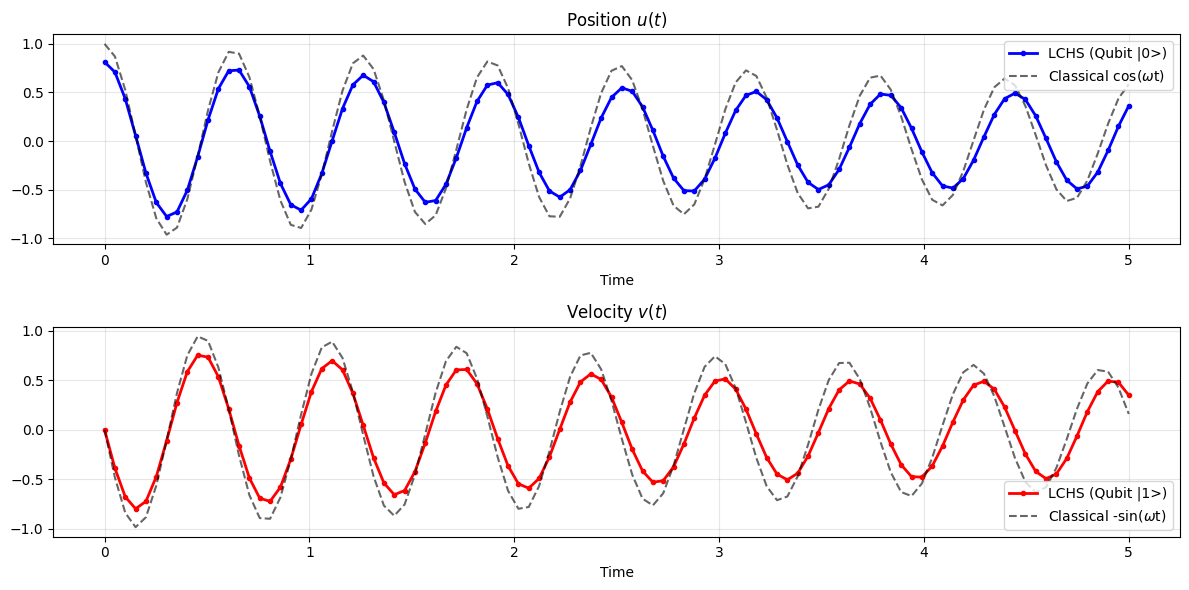
\includegraphics[width=\linewidth]{output_.png}
%     \caption{Position and Velocity of a DHO}
%     \label{fig:DHO}
% \end{figure}


% Figure \ref{fig:DHO} has been generated using the following parameters,
% $\omega = 10.0, 
%     \beta = 0.8,
%     r = 8,
%     r' = 6,
%     N_{dim} = 100,
%     T_{step} = 0.05,
%     n_{steps} = 100, 
%     \gamma=0.2.$

% \subsection*{To-Do, 2/26/26}
%     \begin{enumerate}
%         \item compile with qcvdv and show gate count
%         \item compare qumode energy vs different qubit architectures energy (priotitize superconduncting)
%     \end{enumerate}

\subsubsection{Linear 1st order PDE Example: Discretized One-dimensional Heat Equation}

Consider one-dimensional (1D) heat equation
\begin{align}
    \frac{\partial u(x,t)}{\partial t} = \alpha \frac{\partial^2 u(x,t)}{\partial x^2}
\end{align}
where $\alpha$ (or often written in a squared constant) is called the thermal diffusivity of a length-$L$ rod. Its initial condition is
\begin{align*}
    u(x,0) = f(x), 0<x<L.
\end{align*}
And we start with the easiest boundary condition, a homogeneous Dirichlet boundary condition
\begin{align*}
    u(0,t) = u(L,t) = 0, t>0.
\end{align*}

With a 6-point (2 end-points, $x_0$ and $x_5$ are fixed by the boundary condition) second order central difference approximation
\begin{align*}
    \frac{\partial^2 u(x,t)}{\partial x^2} \bigg\rvert_{x_j} \approx \frac{u(x_{j+1})-2u(x_{j}) + u(x_{j-1})}{h^2}
\end{align*}
we have
\begin{align}
    \frac{\dd}{\dd t}
    \begin{bmatrix}
        u(x_1,t) \\ u(x_2,t) \\ u(x_3,t) \\ u(x_4,t)
    \end{bmatrix}
    = -\frac{\alpha}{h^2} 
    \begin{bmatrix}
        2 &-1 &0 &0 \\ -1 &2 & -1 &0 \\ 0 &-1 &2 &-1 \\ 0 &0 &-1 &2
    \end{bmatrix}
    \begin{bmatrix}
        u(x_1,t) \\ u(x_2,t) \\ u(x_3,t) \\ u(x_4,t)
    \end{bmatrix}, u(x,0) = f(x)
\end{align}
Adopting the convention that $q_0$ is the least significant qubit, the $4\times 4$ Dirichlet Laplacian has the Pauli decomposition
\begin{align}
    T_4
    &=
     \begin{bmatrix}
        2 &-1 &0 &0 \\ -1 &2 & -1 &0 \\ 0 &-1 &2 &-1 \\ 0 &0 &-1 &2
    \end{bmatrix} \\
    &=
    2 I^{\otimes 2} - X_0 - \frac{1}{2} \left( X_1 X_0 + Y_1 Y_0 \right).
\end{align}
For this two-qubit example, $A = \frac{\alpha}{h^2} T_4$. Since $A$ is real symmetric,
\begin{align}
    L &= \frac{A+A^\dagger}{2} = A,\quad    H = \frac{A-A^\dagger}{2i} =  \mathbf{0}
\end{align}

% This problem requires 2 qubits. Since there are no $H$, it also doesn't require any product formula decomposition. The unitary is 
% \[
%     e^{-it(\hat{x}\otimes I_0 I_1)}e^{-it(\hat{x}\otimes I_0 X_1)} e^{-it( \frac{1}{2}\hat{x}\otimes X_0\otimes X_1)}e^{-it( \frac{1}{2}\hat{x}\otimes Y_0\otimes Y_1)}
% \]

% This requires 4 CNOT, 1 CV displacement, and 3 hybrid gates. All the hybrid gates are conditional momentum boost gates, $D(i\alpha_k t)$, where $\alpha_k$ is the coefficient for the Pauli strings. 

% \textcolor{blue}{
% \begin{enumerate}
%     \item Suppose we discretize the domain into $N= 2^m$ data points, what is the Pauli representation for $T$? Does it still give a Pauli sum representation for $L$ where all Paulis are mutually commuting with each other? If not, how many commuting groups of Paulis are there? The idea is that all Paulis within a group are all commuting so they can be performed in a single Trotter step. Then the total number of Trotter steps needed is only equal to the number of non-commuting groups. \textcolor{black}{``done"}
%     \item One can think about mapping the system itself to another oscillator, and synthesize the required non-Gaussian unitary operator using elementary gate set from ISA? One recent paper developed a new method to synthesize multi-qumode non-Gaussian entangling operation https://arxiv.org/abs/2512.19582.\textcolor{black}{``done"}
%     \item Insert a table, summarize the qubit and qumode count, gate count, runtime, as a function of simulation accuracy, time, and diffusion constant. \textcolor{black}{``done"}
%     \item Do the same for the 2D heat equations. \textcolor{black}{``done"}
% \end{enumerate}
% }
To generalize the Pauli decomposition, let $N=2^m$ denote the number of interior grid points and label the computational basis by the binary-encoded site index $\{\ket{x}\}_{x=0}^{N-1}$. The Dirichlet Laplacian on this register is
\begin{align}
    T_m
    =
    2I^{\otimes m}
    -
    \sum_{x=0}^{N-2}\left(\ketbra{x}{x+1}+\ketbra{x+1}{x}\right).
\end{align}
An exact carry-chain decomposition of $T_m$ is
\begin{align}
    T_m = 2I^{\otimes m} - \sum_{c=0}^{m-1} H_c,
    \qquad
    H_c = \sigma_c^+ \prod_{j=0}^{c-1}\sigma_j^- + \sigma_c^- \prod_{j=0}^{c-1}\sigma_j^+,
\end{align}
where
\[
\sigma_j^\pm := \frac{X_j \mp iY_j}{2}.
\]
The operator $H_c$ collects all nearest-neighbor transitions whose binary addition by one ends with a carry chain of length $c$. The first three terms are
\begin{align}
    H_0 &= X_0, \\
    H_1 &= \frac{1}{2}\left(X_1X_0 + Y_1Y_0\right), \\
    H_2 &= \frac{1}{4}\left(X_2X_1X_0 - X_2Y_1Y_0 + Y_2X_1Y_0 + Y_2Y_1X_0\right).
\end{align}
Thus, the two-qubit example above is simply $T_4 = 2I^{\otimes 2} - H_0 - H_1$.

Since $A = \frac{\alpha}{h^2}T_m$ and $H=0$, the hybrid evolution for one Trotter step $\delta t=t/n$ is
\begin{align}
    \mathcal U(\delta t)
    =
    \exp\!\left(-i\theta\,\hat x \otimes T_m\right),
    \qquad
    \theta := \frac{\alpha t}{nh^2}.
\end{align}
Using a first-order product formula,
\begin{align}
    \mathcal U(\delta t)
    \approx
    e^{-i2\theta\,\hat x \otimes I^{\otimes m}}
    \prod_{c=0}^{m-1}
    e^{i\theta\,\hat x \otimes H_c}.
\end{align}
If each $H_c$ is further expanded into Pauli strings,
\[
H_c = \sum_{\ell=1}^{2^c}\gamma_{c,\ell}P_{c,\ell},
\]
then every factor $e^{i\theta\,\hat x\otimes P_{c,\ell}}$ can be synthesized by standard basis changes, a parity-CNOT ladder on the support of $P_{c,\ell}$, and a single CV-controlled phase/displacement on the oscillator. In this naive first-order implementation, one Trotter step contains
\[
1+\sum_{c=0}^{m-1}2^c = N
\]
exponentials in total: one unconditional oscillator phase from the identity term and $N-1$ nontrivial hybrid Pauli exponentials. Since the Pauli strings appearing in $H_c$ have weight $c+1$, the associated two-qubit entangling overhead per Trotter step scales as $\mathcal O(N\log N)$ before commuting-group or hardware-specific optimizations.


Alternatively, we can couple the system oscillator to an ancilla oscillator, in which case the ancilla oscillator encodes the spatial basis $x$ in the position operator $\hat x_2$. Then the heat equation becomes
\cr{The equation below describes free-space heat evolution on $\mathbb{R}$; it does not by itself impose homogeneous Dirichlet boundary conditions on a finite interval.}
\begin{align}
    \frac{\dd \mathbf{u}}{\dd t} = -\alpha \hat p_2^2\mathbf{u}
\end{align}
where $\mathbf{u}:=\int u(x,t)\ket{x}\dd x=\ket{\psi}_{\rm osc_1}\ket{u(t)}_{\rm osc_2}$. This qumode embedding scheme is already known \cite{Jin_2024}. However, we can prepare the initial state $\mathbf{u}(t=0)$ using our proposed methodology from~\ref{ss:state-prep}. Then from theorem~\ref{thm: state-prep}, we can obtain the evolution:
\begin{align}
    \ket{u(t)} &= (\bra{\phi}_{\rm osc}\otimes\mathbb{I)}\hat{U}(\ket{\psi}_{\rm osc}\otimes\ket{u_0}_{\rm anc})
\end{align}

where $\hat{U}:=R(-\frac{\pi}{2})e^{-i\alpha t\hat{x}_1\otimes \hat{x}_2^2}R(\frac{\pi}{2})$ with $e^{-i\alpha t\hat{x}_1\otimes \hat{x}_2^2}$ being the qubic-QND gate~\cite{Hanamura_2024}. This requires two additional ancilla modes.
\cb{If this subsection is kept, it should explicitly say whether it targets the unbounded-line heat equation or add the missing boundary/domain construction needed for the finite-interval Dirichlet problem.}














\subsubsection{Example: Two dimensional Heat Equation}
Two dimensional heat equation
\begin{align}
    \frac{\partial u(x,y,t)}{\partial t} = \alpha \left(\frac{\partial^2 u(x,y,t)}{\partial  x^2}  + \frac{\partial^2 u(x,y,t)}{\partial y^2} \right), u(x,y,0) = f(x,y)
\end{align}
for $0<x<a$ and $0<y<b$. With homogeneous Dirichlet boundary conditions
\begin{align}
    u(0,y,t) &= u(a,y,t) = 0 \leq y \leq b, t \geq 0 \\
    u(x,0,t) &= u(x,b,t) = 0 \leq x \leq a, t \geq 0
\end{align}

Again, using central difference method, we have
\begin{align}
    \frac{\dd u_{i,j}(t)}{\dd t} \approx \frac{u_{i+1,j}(t)- 2 u_{i,j}(t)+u_{i-1,j}(t)}{h_x^2} + \frac{u_{i,j+1}(t)- 2 u_{i,j}(t)+u_{i,j-1}(t)}{h_y^2} 
\end{align}
where $u_{i,j}(t) = u(x_i, y_j, t)$.

Let $M$ be the number of interior points (boundary points are determined by boundary condition) 
\begin{align}
    M = \lceil a/h_x -1 \rceil \cdot \lceil b/h_y - 1\rceil.
\end{align}
Suppose there 2 interior points in $x$-direction and 4 interior points in $y$-direction, we denote
\begin{align}
    u_1 (t) = u(x_1, y_1, t), u_2 (t) = u(x_1, y_2, t), \dots \\
    u_5 (t) = u(x_2, y_1, t), u_6 (t) = u(x_2, y_2, t),  \dots
\end{align}
Note that in this scheme, the neighbor point in $y$ direction is $\pm 1$ indices, but neighbor in $x$ direction is $\pm  \lceil b/h_y - 1\rceil$ indices.

For the form of $u_t = -A u(t)$, in our ordering scheme $A_{k,k} = \frac{2}{h_x^2}+\frac{2}{h_y^2}$, the neighbor in $x$ direction is on the super and sub diagonal $A_{k\pm 1, k} = - \frac{1}{h_y^2}$, and the neighbor in $y$ direction is $A_{k, k \pm 4} = - \frac{1}{h_x^2}.$

An example coefficient matrix is
\[
    A =
    \left(
    \begin{array}{cccccccc}
    \frac{2}{h_x^2}+\frac{2}{h_y^2} & -\frac{1}{h_y^2} & 0 & 0 & -\frac{1}{h_x^2} & 0 & 0 & 0 \\[4pt]
    -\frac{1}{h_y^2} & \frac{2}{h_x^2}+\frac{2}{h_y^2} & -\frac{1}{h_y^2} & 0 & 0 & -\frac{1}{h_x^2} & 0 & 0 \\[4pt]
    0 & -\frac{1}{h_y^2} & \frac{2}{h_x^2}+\frac{2}{h_y^2} & -\frac{1}{h_y^2} & 0 & 0 & -\frac{1}{h_x^2} & 0 \\[4pt]
    0 & 0 & -\frac{1}{h_y^2} & \frac{2}{h_x^2}+\frac{2}{h_y^2} & 0 & 0 & 0 & -\frac{1}{h_x^2} \\[4pt]
    -\frac{1}{h_x^2} & 0 & 0 & 0 & \frac{2}{h_x^2}+\frac{2}{h_y^2} & -\frac{1}{h_y^2} & 0 & 0 \\[4pt]
    0 & -\frac{1}{h_x^2} & 0 & 0 & -\frac{1}{h_y^2} & \frac{2}{h_x^2}+\frac{2}{h_y^2} & -\frac{1}{h_y^2} & 0 \\[4pt]
    0 & 0 & -\frac{1}{h_x^2} & 0 & 0 & -\frac{1}{h_y^2} & \frac{2}{h_x^2}+\frac{2}{h_y^2} & -\frac{1}{h_y^2} \\[4pt]
    0 & 0 & 0 & -\frac{1}{h_x^2} & 0 & 0 & -\frac{1}{h_y^2} & \frac{2}{h_x^2}+\frac{2}{h_y^2}
    \end{array}
    \right).
\]

The Pauli decomposition is
\begin{align}
    A &= \frac{1}{h_y^2} I \otimes T + \frac{2}{h_x^2} I_0I_1I_2 - \frac{1}{h_x^2} X_0 I_1 I_2 \\
    &= \frac{1}{h_y^2} \left[ 2 I_0I_1I_2 - I_0I_1 X_2 - \frac{1}{2} \left( I_0X_1 X_2 + I_0Y_1 Y_2 \right) \right] + \frac{2}{h_x^2} I_0I_1I_2 - \frac{1}{h_x^2} X_0I_1 I_2 \\
    &= \left( \frac{2}{h_y^2} + \frac{2}{h_x^2} \right) I_0 I_1 I_2 - \frac{1}{h_y^2} \left( I_0I_1 X_2 - \frac{1}{2} \left( I_0X_1 X_2 + I_0Y_1 Y_2 \right) \right) - \frac{1}{h_x^2} X_0I_1 I_2 
\end{align}

We take a qubit register of $m$ qubits and divide it into two subregisters of $m_x$ and $m_y$ qubits. We label them as $X$ register and $Y$ register. If we choose arbitrary grid resolutions on both dimensions so that we have $M_x = 2^{m_x}$ points along the $x$-dimension and $M_y = 2^{m_y}$ points along the $y$-dimension, then we can map the system to the subregisters. The 2D Laplacian operator $A$ is then defined by: 
$$A = \frac{1}{h_x^2} (T_x \otimes I^{\otimes m_y}) + \frac{1}{h_y^2} (I^{\otimes m_x} \otimes T_y)$$
where $T_x$ and $T_y$ are the 1D discrete Laplacian operators of dimension $2^{m_x}$ and $2^{m_y}$, respectively. Since $T_x$ and $T_y$ are supported on two disjoint set of qubits, they commute with each other, $[T_x,T_y]=0.$ Then, 

{\color{red}
\[
\mathcal U(\delta t)=\exp\left[\frac{1}{h_x^2} (T_x \otimes I^{\otimes m_y})\right] \exp\left[\frac{1}{h_y^2} (I^{\otimes m_x} \otimes T_y)\right]
\]
}
\cb{Since the two Kronecker-sum terms commute, the corrected hybrid evolution should be}
{\color{blue}
\begin{equation}
\mathcal U(\delta t)=
\exp\left[-i\alpha\delta t\,\hat x\otimes \frac{T_x \otimes I^{\otimes m_y}}{h_x^2}\right]
\exp\left[-i\alpha\delta t\,\hat x\otimes \frac{I^{\otimes m_x} \otimes T_y}{h_y^2}\right].
\end{equation}
}

Thus, one 2D Trotter step factorizes into two commuting 1D heat-equation factors. To avoid redundancy, we skip the circuit breakdown and proceed to the $d$-dimensional generalization.

\cb{(...) Numerical experiment to add: benchmark at least one square grid and one rectangular grid, and report fidelity, post-selection probability, CV cutoff, Trotter steps, and gate counts under the corrected commuting-factor evolution above.}

\cb{(...) Theory check to add: verify whether the CD-gate angles admit a binary pattern that reduces the count from $2^m$ to $m$, and compare the resulting scaling with the best known heat-equation and HHL-style baselines.}


\subsubsection{Example: d-dimensional Heat Equation}

Let $\Omega \subset \mathbb{R}^d$ be a $d$-dimensional rectangular domain defined by:
$$\Omega = \{ (x_1, x_2, \dots, x_d) \in \mathbb{R}^d : 0 < x_i < L_i \quad \text{for } i = 1, \dots, d \}$$
The boundary of the domain is denoted by $\partial\Omega$. Then the evolution of the temperature field $u(\mathbf{x}, t)$ is governed by the $d$-dimensional heat equation:
\begin{align}
    \frac{\partial u(\mathbf{x}, t)}{\partial t} = \alpha \sum_{i=1}^{d} \frac{\partial^2 u}{\partial x_i^2} u(\mathbf{x}, t), \quad \mathbf{x} \in \Omega, \quad t > 0
\end{align}
We impose homogeneous Dirichlet boundary conditions on all $2d$ faces of the hyper-prism:
$$u(\mathbf{x}, t) = 0, \quad \mathbf{x} \in \partial\Omega, \quad t \geq 0$$
For each dimension $i \in \{1, \dots, d\}$:
\begin{align*}
    u(x_1, \dots, x_i=0, \dots, x_d, t) &= 0 \\
    u(x_1, \dots, x_i=L_i, \dots, x_d, t) &= 0
\end{align*}
The state of the system at $t=0$ is given by the initial distribution function $f(\mathbf{x})$:
$$u(\mathbf{x}, 0) = f(x_1, x_2, \dots, x_d), \quad \mathbf{x} \in \Omega$$

This becomes $d$ copies of the 1D carry-chain construction, one for each coordinate register. Consequently, the first-order hybrid resource count grows linearly in $d$: the total number of nontrivial Pauli exponentials per Trotter step is the sum of the 1D counts from each dimension, and the same linear-in-$d$ scaling carries over to the associated qubit entangling overhead.



% We note here that in CV Schrodingerization, we require $d+1$ qumodes, $d$ two-mode Gaussian gates, and $d$ cubic non-Gaussian gates, whereas our proposed algorithm requires only $1$ qumode, $\mathcal{O}\!\left(\frac{t^{1+1/p}d\log N}{{\epsilon_t}^{1/p}}\right)$ CD gates, and no two- or multi-mode gates.







%%%%%%%%%%%%%%%%% Implementations Starts %%%%%%%%%%%%%%%%%%%%%
\section{Implementation and experiment set-ups (MZ)}

\cr{This section currently switches from the theorem-level evolution $e^{-iT(\hat x\otimes L+I\otimes H)}$ to the implementation formula $e^{-iT\hat x\otimes A}$. Those expressions coincide only when $H=0$.}
\cb{For the present working-paper version, this section should be read as the validated heat-equation specialization with $H=0$, so $A=L$ and the implemented map reduces to the theorem-level construction. The nonzero-$H$ implementation should be added later by Trotterizing $e^{-iT(\hat x\otimes L+I\otimes H)}$.}
\cb{Throughout the paper we use the $\hbar=2$ convention. The corresponding $\hbar=1$ formulas used by the numerical backends are recorded in the appendix for implementation convenience.}

The implemented hybrid map for runtime $T$ is the CV-sandwich operator
{\color{red}
\begin{equation}
K(T)=\bra{\phi_r}\,e^{-iT\,\hat{x}\otimes A}\,\ket{\psi_{r,r',\beta}},
\end{equation}
}
\cb{For the heat-equation numerics presently implemented in the code, the map should be written as}
{\color{blue}
\begin{equation}
K(T)=\bra{\phi_r}\,e^{-iT\,\hat{x}\otimes L}\,\ket{\psi_{r,r',\beta}},
\qquad H=0,
\label{eq:impl-map}
\end{equation}
}
where the post-selection state is a squeezed vacuum
\begin{equation}
\ket{\phi_r}=S(r)\ket{0},
\label{eq:impl-post}
\end{equation}
and the preparation state is a squeezed finite Fock superposition
\begin{equation}
\ket{\psi_{r,r',\beta}}=S(r')\sum_{n=0}^{N_{\rm max}-1} C_n\ket{n}.
\label{eq:impl-prep}
\end{equation}
Here $N_{\rm max}$ is the number of retained coefficients.

For a specific initial vector $\bm{u}(0)$, the post-selected DV output is
$\bm{u}_{\mathrm{cv}}=K(T)\bm{u}(0)$ and the reference is
$\bm{u}_{\mathrm{ref}}=e^{-AT}\bm{u}(0)$.
We report the state fidelity
\begin{equation}
F=\left|\frac{\langle\bm{u}_{\mathrm{cv}},\bm{u}_{\mathrm{ref}}\rangle}
{\|\bm{u}_{\mathrm{cv}}\|\;\|\bm{u}_{\mathrm{ref}}\|}\right|^2,
\label{eq:impl-fidelity}
\end{equation}
and the post-selection probability
\begin{equation}
p_{\mathrm{post}}=\|\bm{u}_{\mathrm{DV,post}}\|_2^2,
\label{eq:impl-ppost}
\end{equation}
where $\bm{u}_{\mathrm{DV,post}}$ denotes the DV-register amplitudes immediately after projecting
the CV mode onto $\bra{\phi_r}$.


















\subsection{CV state preparation}
\label{ss:cv-prep}
We use a near-optimal kernel branch parameterized by $0<\beta<1$:
\begin{equation}
f_\beta(k)=\frac{e^{2^\beta}}{2\pi\,e^{(1+ik)^\beta}},
\qquad
g_\beta(k)=\frac{f_\beta(k)}{1-ik}.
\label{eq:impl-kernel}
\end{equation}
Let $\sigma=e^r$ and $\sigma'=e^{r'}$ denote squeezing widths.
Under the paper convention $\hbar=2$, the coefficient integral is
\begin{equation}
C_n \propto \int_{-\infty}^{\infty}
H_n\!\left(\frac{k}{\sigma'}\right)\,
g_\beta(k)\,
e^{-\gamma k^2}\,dk,
\qquad
\gamma=e^{-2r'}-e^{-2r},
\label{eq:impl-coeff-explicit}
\end{equation}
where $H_n(\cdot)$ is the physicists' Hermite polynomial. \cb{The numerically implemented $\hbar=1$ version of this formula is listed in the appendix.} The integral is evaluated numerically using Gaussian quadrature. The state $\ket{\psi_{\mathrm{finite}}}=\sum_{n=0}^{N_{\rm max}-1}C_n\ket{n}$
is prepared using both variational hybrid ansatz and Givens synthesis (Law--Eberly~\cite{law1996arbitrary}). The variational ansatz is achieved through the SNAP-displacement ansatz in \cite{heeres2015cavity, Krastanov2015},
\begin{equation}
U_{\mathrm{SNAP+D}}=\prod_{\ell=1}^{L}D(\alpha_\ell)\,\mathrm{SNAP}(\bm{\theta}_\ell),
\end{equation}
optimized for
\begin{equation}
\max_{\{\alpha_\ell,\bm{\theta}_\ell\}}
\left|\bra{\psi_{\mathrm{finite}}}
U_{\mathrm{SNAP+D}}\ket{0}\right|^2.
\end{equation}

On the other hand, The Givens method prepares $\ket{\psi_{\mathrm{finite}}}=\sum_{n=0}^{N-1}C_n\ket{n}$
from the vacuum $\ket{0}$ using $N-1$ analytically determined rotation steps, without optimization. For Givens rotation, we define the two-level rotation acting on adjacent Fock levels $\ket{n}$, $\ket{n+1}$:
\begin{equation}
G(n,n{+}1;\theta,\varphi)
=\begin{pmatrix}\cos\theta & -e^{-i\varphi}\sin\theta\\
e^{i\varphi}\sin\theta & \cos\theta\end{pmatrix}
\oplus I_{\perp},
\label{eq:givens-rotation}
\end{equation}
where the $2\times2$ block acts on the $\{\ket{n},\ket{n+1}\}$ subspace
and $I_\perp$ is the identity on all other Fock levels.
Any $N$-component target state can be factored as
\begin{equation}
\ket{\psi_{\mathrm{finite}}}
=G(N{-}2,N{-}1;\theta_{N-1},\varphi_{N-1})\cdots G(1,2;\theta_2,\varphi_2)
\,G(0,1;\theta_1,\varphi_1)\,\ket{0},
\label{eq:givens-decomposition}
\end{equation}
where the angles $\{(\theta_k,\varphi_k)\}_{k=1}^{N-1}$ are computed
recursively from the coefficients $C_n$ by a top-down elimination. On a coupled qubit--oscillator platform, a Law--Eberly synthesis alternates single-qubit rotations that set relative amplitudes/phases and a calibrated qubit--oscillator exchange interaction that transfers
population between adjacent Fock levels.
The exchange dynamics are generated in~\cite{jaynes2005comparison},
\begin{equation}
H_{\mathrm{JC}} = \hbar\Omega(t)\bigl(\sigma_- a^\dagger + \sigma_+ a\bigr),
\label{eq:jc-hamiltonian}
\end{equation}
which couples $\ket{e,n}\leftrightarrow\ket{g,n{+}1}$ at the $\sqrt{n+1}$-dependent rate
$\Omega_{n}=\Omega_0\sqrt{n+1}$.
Importantly, a single resonant JC ``swap'' pulse is not photon-number selective by itself; the
effective selectivity required by the Givens factorization is achieved in practice by
hardware calibration and, when available, photon-number-resolved qubit control in the dispersive regime. A representative experimental demonstration of deterministic resonator-state synthesis using such calibrated
sequences is in~\cite{hofheinz2009synthesizing}.







\subsection{Gate-level compilation of hybrid evolution}
\label{sec:impl-trotter}
\cr{The statement below is only consistent with the current validated code path after restricting to the heat-equation case $H=0$.}
\cb{For the present implementation, let $L=\sum_m c_m P_m$ denote the Pauli decomposition of the heat-equation generator. Then we use a first-order product formula over $N_t$ time slices:}
\begin{equation}
e^{-iT\,\hat{x}\otimes L}
\approx
\left(\prod_m e^{-i\Delta t\,c_m\hat{x}\otimes P_m}\right)^{N_t},
\qquad
\Delta t=\frac{T}{N_t}.
\label{eq:impl-trotter}
\end{equation}
Each Pauli term is compiled by a basis change $B_m$ (diagonalize $P_m$ into $Z$-basis)
followed by a parity mapping $C_m$ onto a target qubit $t$:
\begin{equation}
e^{-i\Delta t\,c_m\hat{x}\otimes P_m}
=
B_m^\dagger C_m^\dagger\;
e^{-i\Delta t\,c_m\hat{x}\otimes Z_t}\;
C_m B_m.
\label{eq:impl-parity}
\end{equation}
The primitive hybrid interaction $e^{-i\lambda \hat{x}\otimes Z_t}$ is implemented as a conditional displacement
with amplitude $\alpha=-i\lambda/\sqrt{2}$.










% %%%%%%%%%%%%%%%%% Experiments Starts %%%%%%%%%%%%%%%%%%%%%
\section{Experiments (MZ)}

\cb{(...) 1D heat experiments to add: reproduce the same canonical parameter set in QuTiP, bosonic compilation, and sweep scripts for at least three grids, and report fidelity, post-selection probability, truncation parameters, and gate counts.}

\cb{(...) 2D heat experiments to add: include at least one square-grid and one rectangular-grid instance, using the corrected commuting-factor evolution, with the same metrics plus a brief comparison against classical finite-difference propagation.}

\cb{(...) Scaling table to add: summarize how the chosen best parameter set changes with runtime $T$, diffusion constant $\alpha$, grid size, Fock cutoff, coefficient count, and Trotter step count.}

% n_qubits=2, n_fock=64, n_coeff=48
% r=6, r'=4, beta=0.3, T=1.0, trotter_steps=10

% [injection] post_prob=2.764643e-01, layout=fock_major
%   fidelity vs classical: 0.97791933
%   fidelity vs qutip    : 0.99995970
%   state-prep metadata  : {'stateprep_seed_fidelity': 1.0}
%   depth=152, size=234
%   count_ops={'h': 100, 'cx': 40, 'rz': 40, 'cD': 30, 'D': 20, 'S': 2, 'initialize': 1, 'x': 1}

% [snap_d] post_prob=1.897904e-01, layout=fock_major
%   fidelity vs classical: 0.98788789
%   fidelity vs qutip    : 0.99176145
%   state-prep metadata  : {'stateprep_seed_fidelity': 0.728587501621602, 'stateprep_depth': 10.0, 'stateprep_restarts': 2.0}
%   depth=641, size=723
%   count_ops={'SNAP': 480, 'h': 100, 'cx': 40, 'rz': 40, 'D': 30, 'cD': 30, 'S': 2, 'x': 1}

% [Givens] post_prob=2.764643e-01, layout=fock_major
%   fidelity vs classical: 0.97791933
%   fidelity vs qutip    : 0.99995970
%   state-prep metadata  : {'stateprep_analytic_fidelity': 1.0, 'n_active_fock_levels': 48.0, 'n_jc_pulses': 47.0, 'n_qubit_rotations': 47.0}
%   depth=152, size=234
%   count_ops={'h': 100, 'cx': 40, 'rz': 40, 'cD': 30, 'D': 20, 'S': 2, 'initialize': 1, 'x': 1}






















%%%%%%%%%%%%%%%%% Conclusion Starts %%%%%%%%%%%%%%%%%%%%%
\section{Conclusion}









\section{Future Works}





%%%%%%%%%%%%%%%%% Rest %%%%%%%%%%%%%%%%%%%%%
\section{Author Contributions}
If needed


\section{Acknowledgments}

ERD acknowledges fruitful discussions with Kaustubh Chandramouli.


\section{Competing interests}
All authors declare no financial or non-financial competing interests. 




\section{Data and code availability}





\bibliography{refs}
\bibliographystyle{unsrt}


%%%%%%%%%%%%%%%%% Appendix %%%%%%%%%%%%%%%%%%%%%
\appendix
% Some LCHS basics if needed
\section{Appendix}
\subsection{Complementary (Homogeneous) Solution  $\Tcal e^{- \int^t_0 A(s) \dd s}u_0$}

\begin{remark}
With a quadrature rule, the goal is to find the approximation
\begin{align}
    \int^b_a g(x) \approx \sum_{j=0}^{m-1} w_j g(x_j).
\end{align}
For an integral over $[-1,1]$ with Gaussian quadrature with $m$ nodes, set node $x_j$ to be the root of Legendre polynomial of degree $m$, $P_m(x)$ with weight $w_j = \frac{2}{(1-x^2_j)((P'_m(x_j))^2}$. For a longer interval $[a,b]$, the composite rule is applied by dividing the interval $[a,b]$ into $K$ segments, i.e., $[a+kh, a+(k+1)h]$ where $h = \frac{b-a}{K}$ is the step size. Gaussian quadrature is applied on each shorter interval and it is constructed from that on $[-1,1]$ by a change of variable. That is, the weight $w_j \rightarrow \frac{h}{2}w_j$ and node $x_j \rightarrow \frac{h}{2}x_j + (a+kh) + \frac{1}{2}h$.
\end{remark}


Consider the ODE solution over a truncated finite interval $[-K,K]$ using the composite Gaussian quadrature to discretize the interval. 

The first step is to define
\begin{align}
    g(k) = \frac{1}{C_\beta (1-ik)e^{(1+ik)^\beta}}, \quad U(T,k) = \Tcal e^{-i \int^T_0 (kL(s)+H(s)) \dd s}.
\end{align}
Then,
\begin{align}
    \Tcal e^{-\int^T_0 A(s) \dd s} &= \int_\Rbb g(k) U(T,k) \dd k   && \text{(by LCHS)}    \nonumber \\
    &\approx \int^K_{-K} g(k) U(T,k) \dd k      && \text{(truncation)} \nonumber \\
    &= \sum_{m = -K/h_1}^{K/h_1-1} \int^{(m+1)h_1}_{mh_1} g(k)U(T,k) \dd k    && \text{(divide to shorter intervals)}\nonumber \\
    &\approx \sum_{m=-K/h_1}^{K/h_1 -1}\sum_{q=0}^{Q-1} c_{q,m}U(T,k_{q,m})   && \text{(Gaussian quadrature in each interval)} \label{eq:homo-gauss1}\\
    &= \sum_{j=0}^{M-1} c_j U(T,k_j)  && \text{(simplified notation)} 
\end{align}
where $h_1$ is the step size in the composite Gaussian quadrature, $Q$ is the number of nodes in each interval $[mh_1, (m+1)h_1]$, $k_{q,m}$ is a Gaussian node, $c_{q,m} = w_qg(k_{q,m})$, $w_q$ is a Gaussian weight (which does not depend on the choice of $m$), and $M$ is the overall number of the nodes (or unitaries). 

% \begin{align}
%     \Tcal e^{-\int^T_0 A(s) \dd s} = \int_\Rbb g(k) U(T,k) \dd k  \approx \int^K_{-K} g(k) U(T,k) \dd k     = \sum_{j=0}^{M-1} c_j U(T,k_j) 
% \end{align}

\begin{assumption}
    Assume $K$ and $h_1$ are chosen so that $K/h_1$ is an integer.
\end{assumption}

To bound the truncation error by $\epsilon > 0$, it suffices to choose 
\begin{align*}
    K = \Ocal \left(\left(\log(1/\epsilon)\right)^{1/\beta}\right)
\end{align*}
To bound the quadrature error by $\epsilon > 0$, it suffices to choose
\begin{align}
    h_1 = \frac{1}{eT \max_t \|L(t)\|}, \ Q = \left\lceil \frac{1}{\log 4}  \log\left( \frac{8}{3C_\beta} \frac{K}{\epsilon} \right)\right\rceil = \Ocal\left(\log \frac{1}{\epsilon}\right), \label{eq:homo-hq}
\end{align}
and the overall number of unitaries in the summation formula is
\begin{align}
    M = \frac{2KQ}{h_1} = \Ocal\left( T \max_t \|L(t)\|\left(\log \frac{1}{\epsilon}\right)^{1+1/\beta} \right)
\end{align}




For the specific value of $K$, note that in Eq. (176) in~\cite{LCHS2}, we have 
\begin{align}
\left\|\int_\Rbb g(k) U(T,k) \dd k  -\int^K_{-K} g(k) U(T,k) \dd k  \right\| &\leq \frac{2^{B+1}B!}{C_\beta (\cos(\beta \pi /2))^B} \frac{1}{K} e^{-\frac{1}{2}K^\beta \cos(\beta \pi /2)} \leq \epsilon \nonumber \\
\ln \left( \frac{2^{B+1}B!}{C_\beta (\cos(\beta \pi /2))^B}\right)  + \ln(1/ \epsilon)  &\leq \ln(K) + \frac{1}{2}K^\beta \cos(\beta \pi /2) \\
2\cdot \frac{\ln \left( \frac{2^{B+1}B!}{C_\beta (\cos(\beta \pi /2))^B}\right)  + \ln(1/ \epsilon) - \ln(K)}{ \cos(\beta \pi /2)} &\leq K^\beta
\end{align}
where $B = \lceil 1/\beta \rceil$








%%%%%%%%%%%%%%%%%%%

\subsection{Inhomogeneous Term $\int^t_0 \Tcal e^{-\int^t_s A(s')\dd s'}b(s) \dd s$}


The discretization of the inhomogeneous term is
{\footnotesize
\begin{align}
    &\quad \int^T_0 \Tcal e^{-\int^T_s A(s')\dd s'}b(s) \dd s  \nonumber \\
    &= \int^T_0 \int_\Rbb \frac{f(k)}{1-ik} U(T,s,k) b(s) \dd k \dd s   && \text{(by LCHS Eq.~\eqref{eq:LCHS-sol-homo})}    \nonumber \\
    &\approx \int^T_0  \sum_{m_1 = -K/h_1}^{K/h_1 - 1} \sum_{q_1 = 0}^{Q_1 - 1} c_{q_1, m_1} U(T, s, k_{q_1, m_1}) b(s) \dd s        &&\text{(by 
 Eq.~\eqref{eq:homo-gauss1})}   \nonumber \\
    &\approx \sum_{m_2 = 0}^{T/h_2 - 1} \sum_{q_2 = 0}^{Q_2 - 1}    \sum_{m_1 = -K/h_1}^{K/h_1 - 1} \sum_{1_1 = 0}^{Q_1 - 1} c'_{q_2, m_2} c_{q_1, m_1} U(T, s_{q_2, m_2}, k_{q_1, m_1} ) \ket{b(s_{q_2, m_2})}        &&\text{(composite Gaussian quadrature) } \\
    &= \sum_{j'=0}^{M'-1} \sum_{j = 0}^{M-1} c'_{j'} c_j U(T, s_{j'}, k_j)\ket{b(s_{j'})} && \text{(simplified notation)} \label{eq:inhomo}
\end{align}
}
where $ U(T,s,k) = \Tcal e^{-i\int^T_s (kL(s') + H(s') \dd s' }$, $h_2$ is the step size for the discretization of the time integral, $Q_2$ is the number of Gaussian quadrature nodes, $s_{q_2, m_2}$ is a node, $c'_{q_2,m_2} = w'_{q_2}\|b(s_{q_2, m_2})\|$, the $w'_{q_2}$ is a Gaussian weight. The $\ket{b}$ implies that it is the normalized vector $b/\|b\|$.

Let 
\begin{itemize}
    \item $\Lambda = \sup_{p \geq 0, t\in [0,T]} \|A^{(p)}\|^{1/(p+1)}$ 
    \item $\Xi = \sup_{p \geq 0, t\in [0,T]} \|b^{(p)}\|^{1/(p+1)}$, where $(p)$ refers to the $p^{th}$-order time derivative
    \item $\|b\|_{L^1} = \int^T_0 \|b(s)\| \dd s$
\end{itemize}
To bound the approximation error of Eq.~\eqref{eq:inhomo} by $\epsilon > 0$, it suffices to choose
\begin{align}
    K = \Ocal\left( \left( \log\left( 1+ \frac{\|b\|_{L^1}}{\epsilon}\right) \right)^{1/\beta} \right), \   h_1 = \frac{1}{eT\max_t \|L(t)\|}, h_2 = \frac{1}{eK(\Lambda+\Xi)}, \label{eq:inhomo-K} \\
    Q_1 = \Ocal\left( \log\left( 1+\frac{\|b\|_{L^1}}{\epsilon} \right) \right), Q_2 = \Ocal\left( \log\left( \frac{T(\Lambda+\Xi)}{\epsilon} \right) \right)
\end{align}
and
\begin{align*}
    M' = \frac{TQ_2}{h_2} = \Ocal\left( TK(\Lambda+\Xi)\log\left( \frac{T(\Lambda+\Xi)}{\epsilon} \right)  \right) = \tilde{\Ocal}\left( T(\Lambda+\Xi) \left( \log\left( 1+ \frac{\|b\|_{L^1}}{\epsilon}\right) \right)^{1/\beta} \log\left(1/\epsilon\right)\right)
\end{align*}

As indicated in Eq. (234) and (235) in~\cite{LCHS2}, we have
\begin{align}
    \|c\|_1 \frac{eT(\Lambda+\Xi)}{4^{Q_2} } &\leq \frac{\epsilon}{2} \nonumber \\
    \frac{1}{ \ln(4)} \ln \left( \|c\|_1 \frac{2eT(\Lambda+\Xi)}{\epsilon} \right) &\leq Q_2,
\end{align}
where $ \|c\|_1 = \Ocal(1)$. For computing $Q_1$, just use the same formula in Eq.~\eqref{eq:homo-hq} but with the $K$ in Eq.~\eqref{eq:inhomo-K}.


\subsection{Summary}
With LCHS, Eq.~\eqref{eq:exp-sol} becomes
\begin{align}
    u(T) \approx \sum_{j=0}^{M-1} c_j U(T,k_j) \ket{u_0}  + \sum_{j'=0}^{M'-1} \sum_{j = 0}^{M-1} c'_{j'} c_j U(T, s_{j'}, k_j)\ket{b(s_{j'})}.
\end{align}
where $ U(T,s,k) = \Tcal e^{-i\int^T_s (kL(s') + H(s')) \dd s' }$ and $U(T,k) = U(T,0,k)$. So, we need oracles circuit to implement the Hamiltonian simulation operator $U(T,s,k)$ and  oracles to encode the coefficients $c$ and $c'$ into amplitudes. Then, use LCU to obtain $u(T)$.




\subsection{Analytical Values of the Expansion Coefficients $C_n$ at limit values of $\beta$}
\label{ss:analytic}
The coefficients are defined by the projection of the signal $g(x)$ onto the Hermite basis:

\begin{equation}
    C_n(\beta) = \mathcal{K}_n \int_{-\infty}^{\infty} \frac{H_n(x/\sigma') e^{-\gamma x^2}}{2\pi e^{-2^\beta} e^{(1+ix)^\beta} (1-ix)} \, \dd x
\end{equation}

where $\mathcal{K}_n = \sqrt{\frac{\sigma}{\sigma'}} \frac{1}{\sqrt{2^n n!}}$ and $\gamma = \sigma'^{-2} - \sigma^{-2}$. We denote the coefficient functions at the limit points as $C_n^{(0)}$ and $C_n^{(1)}$, corresponding to the limits $\beta=0$ and $\beta=1$, respectively.

We employ an explicit polynomial decomposition of the Hermite-Lorentzian kernel. By defining a residual quotient polynomial $Q_{n-1}(x) = [H_n(x/\sigma') - H_n(-i/\sigma')] / (x + i)$, we isolate the singular contribution of the complex pole at $x = -i$.

At the limit $\beta = 0$, the denominator simplifies to a standard complex Lorentzian. The exact closed-form expression is:
\begin{equation}
    C_n^{(0)} = \mathcal{K}_n \left[ \frac{1}{2} H_n\left(-\frac{i}{\sigma'}\right) e^\gamma \text{erfc}(\sqrt{\gamma}) + \frac{i}{2\pi} \int_{-\infty}^{\infty} Q_{n-1}(x) e^{-\gamma x^2} \, \dd x \right]
\end{equation}

For $\beta = 1$, the kernel incorporates a phase shift $e^{-ix}$ and a scaling factor $e^1$. Completing the square in the exponent for the shifted Gaussian ($-\gamma x^2 - ix$) leads to:
\begin{equation}
    C_n^{(1)} = \mathcal{K}_n \left[ \frac{1}{2} H_n\left(-\frac{i}{\sigma'}\right) e^\gamma \text{erfc}\left(\sqrt{\gamma} - \frac{1}{2\sqrt{\gamma}}\right) + \frac{ie}{2\pi} \int_{-\infty}^{\infty} Q_{n-1}(x) e^{-\gamma x^2 - ix} \, \dd x \right]
\end{equation}
The transition from $\beta=0$ to $\beta=1$ effectively shifts the argument of the error function by $\Delta = (2\sqrt{\gamma})^{-1}$.




\subsubsection{Numerical Validation}
The analytical results were compared against direct numerical quadrature using a double-exponential integration scheme with a working precision of 30 decimal places. For the parameter set $\sigma' = 1.2$ and $\sigma = 2.0$ ($\gamma = 4/9$), the agreement is presented in the tables below.




\begin{table}[h!]
\centering
\caption{Comparison of Numerical and Analytical Coefficients for the Lower Bound ($\beta = 0, \gamma = 4/9$)}
\label{tab:lower_bounds}
\begin{tabular}{rll}
\hline
$n$ & Numerical Result & Analytical (Explicit) \\
\hline
0 & 0.3481065885 & 0.3481065885 \\
1 & $0.2335427879i$ & $0.2335427879i$ \\
2 & $-0.0515295394$ & $-0.0515295394$ \\
3 & $-0.0077856810i$ & $-0.0077856810i$ \\
\hline
\end{tabular}
\end{table}





\begin{table}[h!]
\centering
\caption{Comparison of Numerical and Analytical Coefficients for the Upper Bound ($\beta = 1, \gamma = 4/9$)}
\label{tab:upper_bounds}
\begin{tabular}{rll}
\hline
$n$ & Numerical Result & Analytical (Explicit) \\
\hline
0 & 1.1011786413 & 1.1011786413 \\
1 & $-0.3006294949i$ & $-0.3006294949i$ \\
2 & $-0.0943736080$ & $-0.0943736080$ \\
3 & $-0.1769037943i$ & $-0.1769037943i$ \\
\hline
\end{tabular}
\end{table}



As demonstrated in Tables~\ref{tab:lower_bounds} and~\ref{tab:upper_bounds}, the explicit decomposition method maintains a relative error below $10^{-25}$.


\subsection{Translation to the $\hbar=1$ Backend Convention}
\cb{The main text uses the $\hbar=2$ convention. For numerical backend convenience, we record the corresponding $\hbar=1$ formulas used by the QuTiP and bosonic simulation codes.}

\cb{If the paper convention is written with}
{\color{blue}
\[
\hat x_{(2)} = a+a^\dagger,
\]
}
\cb{then the backend convention is}
{\color{blue}
\[
\hat x_{(1)}=\frac{a+a^\dagger}{\sqrt{2}},
\qquad
\hat x_{(2)}=\sqrt{2}\,\hat x_{(1)}.
\]
}

\cb{Accordingly, the coefficient-exponent parameter appearing in the prepared-state overlap changes from}
{\color{blue}
\[
\gamma_{(2)} = e^{-2r'}-e^{-2r}
\]
}
\cb{to}
{\color{blue}
\[
\gamma_{(1)} = \frac{1}{2}\left(e^{-2r'}-e^{-2r}\right)=\frac{\gamma_{(2)}}{2}.
\]
}

\cb{Thus the backend coefficient integral is}
{\color{blue}
\begin{equation}
C_n^{(\hbar=1)} \propto \int_{-\infty}^{\infty}
H_n\!\left(\frac{k}{\sigma'}\right)\,
g_\beta(k)\,
e^{-\gamma_{(1)} k^2}\,dk,
\qquad
\gamma_{(1)}=\frac12\left(e^{-2r'}-e^{-2r}\right).
\end{equation}
}

\cb{Likewise, a hybrid interaction written in the paper convention as}
{\color{blue}
\[
e^{-i\lambda\,\hat x_{(2)}\otimes P}
\]
}
\cb{is implemented in an $\hbar=1$ backend as}
{\color{blue}
\[
e^{-i(\sqrt{2}\lambda)\,\hat x_{(1)}\otimes P},
\]
}
\cb{so the coupling coefficient supplied to the backend must be rescaled by a factor of $\sqrt{2}$.}


\section{Fourier-Laplace Transform}
\cr{The Fourier-Laplace section below is not yet theoretically consistent: the kernel notation mixes $k$ and $z$, the normalization is malformed, and the two-oscillator theorem does not yet match the operator structure being claimed.}
\cb{For the current working-paper version, this section should be treated as exploratory only. A clean revision should use one integration variable, fix the kernel normalization, and derive the two-oscillator sandwich directly from the target Laplace-transform representation before stating a theorem.}

Ref.~\cite{an2024laplacetransformbasedquantum} proposed an LCHS-based Laplace transform QEVT. The theorem is as follows:

Let 
\[
A = L + iH, \quad \text{where} \quad 
L = \frac{A + A^{\dagger}}{2} \succeq 0
\quad \text{and} \quad 
H = \frac{A - A^{\dagger}}{2i}
\]
are both Hermitian matrices. 

For a function 
\[
h(z) = \int_{0}^{\infty} g(t)e^{-zt}\,dt
\]
that can be expressed by a Laplace transformation with \(g(t)\) being its inverse Laplace transform, we have
\[
h(A) = \int_{0}^{\infty} \int_{\mathbb{R}} 
\frac{f(k)g(t)}{1 - ik}\, e^{-it(kL+H)} \, dk \, dt.
\tag{5}
\]

Here
{\color{red}
\[
f(k) = \frac{1}{2\pi e^{-2\beta} e^{(1+iz)\beta}}, 
\qquad \beta \in (0,1).
\]
}
\cb{If this appendix keeps the same near-optimal kernel convention as the main text, it should instead use}
{\color{blue}
\[
f_\beta(k)=\frac{e^{2^\beta}}{2\pi e^{(1+ik)^\beta}},
\qquad
g_\beta(k)=\frac{f_\beta(k)}{1-ik},
\qquad
\beta \in (0,1),
\]
}
\cb{with the same branch choice and normalization used throughout the rest of the paper.}

We propose the CVDV LCHS based Laplace transform theorem as follows:
{\color{red}
\begin{theorem}
\begin{align}
    \ket{u(t)} &= h(A) \ket{u(0)}= \bra{\Phi_{\rm osc_1}}\braket{\Phi_{\rm osc_2}|e^{-i(\hat x_1\otimes \hat x_2\otimes L+\hat{x}_1\otimes \mathbf{I}\otimes H)}|\Psi_{\rm osc_2}}\ket{\Psi_{\rm osc_1}} \\
    &= (\bra{\phi}_{\rm osc_1}\otimes\mathbf{I_{\rm osc_2}}\otimes\mathbf{I}_q) (\mathbf{I_{\rm osc_1}}\otimes\bra{\phi}_{\rm osc_2}\otimes\mathbf{I}_q) e^{-it ( \hat{x} \otimes L+ \mathbf{I}_{\rm osc} \otimes H} (\ket{\psi}_{\rm osc_1}\otimes\ket{\psi}_{\rm osc_2}\otimes\ket{u_0}_q)\\
    &= \left[\int_{\mathbb{R}} \int_{\mathbb{R}} \dd x_1 \dd x_2 \, \phi_1^*(x_1) \psi_1(x_1)   \, \phi_2^*(x_2) \psi_2(x_2)   e^{-it ( xL + H)}\right]\ket{u_0}_q.
\end{align}
\end{theorem}
}
\cb{(...) Replace the theorem above with a fully derived two-oscillator statement after the target Laplace-transform representation is fixed. The revised theorem should specify the joint unitary, both post-selection kernels, the resulting double-integral weight, and the exact conditions under which the construction reproduces $h(A)$.}


\end{document}
